\lab{Algorithms}{Interior Point II}{Interior Point II}
\objective{Learn About Interior Point Methods for Quadratic Constrained Optimization.}

In this lab, we will explore an extension of Interior Point methods to a broader class of
problems, namely quadratic constrained optimization problems.
A \emph{quadratic constrained optimization problem}, also known as a quadratic program,
differs from a linear constrained optimization problem (or linear program) only in that
the objective function is quadratic rather than linear.
We can pose such a problem as follows:
\begin{align*}
\text{minimize }\qquad \frac{1}{2}&x^TQx + c^Tx\\
\text{subject to }\qquad &Ax \geq b,\\
&Gx = h.
\end{align*}
Unlike linear constrained optimization, the optimal point is not guaranteed to be one of the vertices of the
feasible polytope. Thus, any attempt to extend the popular Simplex Algorithm to quadratic
programs would require substantial adjustments, as that algorithm is based crucially on locating and searching through
the vertices of the feasible region. Interior Point methods, however, generalize readily to the situation at hand.
In this lab, you will learn about and implement a primal-dual Interior Point method for quadratic constrained
optimization. You will then explore applications in elastic membrane theory and in finance.

\section*{Quadratic Interior Point Method}
We will restrict our attention to quadratic programs involving positive semidefinite quadratic terms.
(In general, indefinite quadratic objective functions admit many local minima, complicating matters
considerably.) Such problems are called \emph{convex}, since the objective function is convex.
To simplify the exposition, we will also only allow inequality constraints (generalizing to
include equality constraints is not a difficult task). Thus, we have the problem
\begin{align*}
\text{minimize }\qquad \frac{1}{2}&x^TQx + c^Tx\\
\text{subject to }\qquad &Ax \geq b,\\
\end{align*}
where $Q$ is an $n\times n$ positive semidefinite matrix, $x, c \in \mathbb{R}^n$, $A$ is an $m \times n$ matrix,
and $b \in \mathbb{R}^m$.

The Interior Point method we describe here is an adaptation of the method we used with linear
programming. The basic intuition is the same as before: we start at some point in the interior of the
feasible region, and we make a series of steps so that we approach the solution to the KKT conditions
iteratively. Since the the solution to the KKT conditions can be seen as the root of a system of equations,
our first thought might be to use Newton's Method for root-finding. This will not work on its own, however,
because the KKT conditions also require inequality constraints, which will be violated if we blindly apply
Newton's Method. Hence, we make adjustments to our choice of search direction and step size, so that we
respect the constraints while moving closer to the solution of the KKT conditions.

We begin by deriving the KKT conditions for this problem. The first step is to form the Lagrangian function,
which has the form
\[
\mathcal{L}(x,\lambda) = \frac{1}{2}x^TQx + c^Tx - \lambda^T(Ax -b).
\]
We next take the gradient of the Lagrangian with respect to $x$ and set it equal to zero:
\begin{align*}
0 &= \nabla_x \mathcal{L}(x,\lambda)\\
&= Qx + c - A^T\lambda.
\end{align*}
We next write the complementary slackness condition:
\[
(Ax - b)_i\lambda_i = 0, \qquad i=1,2,\ldots,m.
\]
We finish by listing the inequality constraints as well as the nonnegativity constraint for $\lambda$:
\begin{align*}
Ax - b &\geq 0,\\
\lambda &\geq 0.
\end{align*}

What we have now is a mixture of equations and inequalities. We want to express these conditions as a system of equations,
so we introduce a nonnegative slack vector $y$ to change the inequality
\[
Ax - b \geq 0
\]
into an equality
\[
Ax - b - y = 0.
\]
This clearly implies that $y = Ax - b$, so we make this substitution into the complementary slackness conditions.
We obtain the following statement of the KKT conditions:
\begin{align*}
Qx - A^T\lambda + c &= 0,\\
Ax - y - b &= 0,\\
y_i\lambda_i &= 0, \qquad i=1,2,\ldots,m,\\
y,\lambda &\geq 0.
\end{align*}

Define $\mathcal{Y} = \text{diag}(y_1,y_2,\ldots,y_m)$ and $\Lambda = \text{diag}(\lambda_1,\lambda_2,\ldots,\lambda_m)$.
Denote the vector in $\mathbb{R}^m$ consisting entirely of ones by $e$. With this notation, we can define a function
\[
F(x,y,\lambda) =
\begin{bmatrix}
Qx-A^Ty + c\\
Ax-y-b\\
\mathcal{Y}\Lambda e
\end{bmatrix}.
\]
Then our KKT conditions can be expressed succinctly in the following manner:
\begin{align*}
F(x,y,\lambda) &= 0,\\
y,\lambda &\geq 0.
\end{align*}
Our goal is to produce a sequence of points that approach the solution to this system of equations, all the while
respecting the nonnegativity constraints $y,\lambda \geq 0$.

We achieve this goal using largely the same approach our linear programming Interior Point method.
We first apply Newton's method to $F$, obtaining a Newton search direction $(\triangle x, \triangle y, \triangle \lambda)$
that solves the system
\begin{equation}
\begin{bmatrix}
Q & 0 & -A^T\\
A & -I & 0\\
0 & \Lambda & \mathcal{Y}
\end{bmatrix}
\begin{bmatrix}
\triangle x\\
\triangle y\\
\triangle \lambda
\end{bmatrix}
=
\begin{bmatrix}
-Qx + A^T\lambda - c\\
-Ax + y + b\\
-\Lambda\mathcal{Y}e
\end{bmatrix}.
\label{eq:affine}
\end{equation}
We may not be able to step far in this direction without violating the nonnegativity constraints, so we calculate
an improved direction by perturbing the system of equations. This is done by making several small calculations.

First calculate the \emph{duality measure}
\[
\mu = \frac{1}{m}y^T\lambda,
\]
which tells us about how close we are to the optimal point (values closer to zero indicate better proximity to the optimizer).

Next, we calculate a maximal allowed step length in the Newton direction:
\[
\hat{\alpha} = \max \{\alpha \in (0,1] \, | \, (y,\lambda) + \alpha(\triangle y, \triangle \lambda) \geq 0\}.
\]
You can check that this value is given by the minimum of the values
\begin{align*}
\min\left(1, \min_{i : \triangle y_i < 0} - \frac{y_i}{\triangle y_i}\right),\\
\min\left(1, \min_{i : \triangle \lambda_i < 0} -\frac{\lambda_i}{\triangle \lambda_i}\right).
\end{align*}

Continuing on, we compute the Newton duality measure given by
\[
\hat{\mu} = \frac{1}{m}(y + \hat{\alpha}\triangle y)^T(\lambda + \hat{\alpha}\triangle \lambda),
\]
and then the centering parameter
\[
\sigma = \left(\frac{\hat{\mu}}{\mu}\right)^3.
\]

Finally, we obtain our search direction $(\triangle x', \triangle y', \triangle \lambda')$ by solving the perturbed
system
\begin{equation}
\begin{bmatrix}
Q & 0 & -A^T\\
A & -I & 0\\
0 & \Lambda & \mathcal{Y}
\end{bmatrix}
\begin{bmatrix}
\triangle x'\\
\triangle y'\\
\triangle \lambda'
\end{bmatrix}
=
\begin{bmatrix}
-Qx + A^T\lambda - c\\
-Ax + y + b\\
-\Lambda\mathcal{Y}e - \triangle \Lambda\triangle\mathcal{Y}e + \sigma\mu e
\end{bmatrix}.
\label{eq:perturbed}
\end{equation}

Now that we have our search direction, we select a step length. We want to step nearly as far as possible
without violating the nonnegativity constraints. We back off slightly from the maximum allowed step length, however,
because an overly greedy step at one iteration may prevent a decent step at the next iteration. Thus,
we choose our step size
\[
\alpha = \max\{a \in (0,1] \, | \, \tau(y,\lambda) +a(\triangle y', \triangle \lambda') \geq 0\},
\]
where $\tau \in (0,1)$ controls how much we back off from the maximal step length. For now, choose $\tau = 0.9$.
In general, $\tau$ can be made to approach $1$ at each successive iteration, and this may speed up convergence in some cases.

Finally, we step to our new point $(x', y', \lambda')$ using the formula
\[
(x', y', \lambda') = (x, y, \lambda) + \alpha(\triangle x', \triangle y', \triangle \lambda').
\]
This completes one iteration of the algorithm.
We summarize the entire procedure in Algorithm \ref{alg:predcorr}.
\begin{algorithm}
\begin{algorithmic}[1]
\Procedure{Predictor-Corrector Algorithm for QP}{}
    \State \textrm{Choose initial point } $(x_0, y_0, \lambda_0)$.
    \For{$k = 0, 1, 2, \ldots$}
        \State \textrm{Solve \ref{eq:affine} for } $(\triangle x, \triangle y, \triangle \lambda)$.
        \State \textrm{Calculate } $\mu, \hat{\alpha}, \hat{\mu},$\textrm{and} $\sigma$.
        \State \textrm{Solve \ref{eq:perturbed} for } $(\triangle x', \triangle y',\triangle \lambda')$.
        \State \textrm{Calculate the step length } $\alpha$.
        \State $(x_{k+1}, y_{k+1}, \lambda_{k+1}) = (x_k, y_k, \lambda_k) + \alpha(\triangle x', \triangle y', \triangle \lambda').$
    \EndFor
\EndProcedure
\end{algorithmic}
\caption{Predictor-Corrector Algorithm}
\label{alg:predcorr}
\end{algorithm}

As with our Interior Point method for linear constrained optimization, the most expensive part of each iteration
is solving the linear systems \ref{eq:affine} and \ref{eq:perturbed}. Note, however, that these systems both have
the same matrix on the left-hand side. This allows us to factor the matrix just once per iteration, and use the
factorization to solve both systems. A more sophisticated implementation would likely split up these large
systems of equations into a few smaller ones, and then use Cholesky-based factorizations. To simplify matters, we
suggest simply using as a first attempt an LU decomposition on the entire matrix.

As usual, the starting point $(x_0, y_0, \lambda_0)$ has an important effect on the convergence of the algorithm.
The code listed below will calculate an appropriate starting point:
\begin{lstlisting}
def startingPoint(G, c, A, b, guess):
    """
    Obtain an appropriate initial point for solving the QP
    .5 x^T Gx + x^T c s.t. Ax >= b.
    Inputs:
        G -- symmetric positive semidefinite matrix shape (n,n)
        c -- array of length n
        A -- constraint matrix shape (m,n)
        b -- array of length m
        guess -- a tuple of arrays (x, y, l) of lengths n, m, and m, resp.
    Returns:
        a tuple of arrays (x0, y0, l0) of lengths n, m, and m, resp.
    """
    m,n = A.shape
    x0, y0, l0 = guess

    # initialize linear system
    N = np.zeros((n+m+m, n+m+m))
    N[:n,:n] = G
    N[:n, n+m:] = -A.T
    N[n:n+m, :n] = A
    N[n:n+m, n:n+m] = -np.eye(m)
    N[n+m:, n:n+m] = np.diag(l0)
    N[n+m:, n+m:] = np.diag(y0)
    rhs = np.empty(n+m+m)
    rhs[:n] = -(G.dot(x0) - A.T.dot(l0)+c)
    rhs[n:n+m] = -(A.dot(x0) - y0 - b)
    rhs[n+m:] = -(y0*l0)

    sol = la.solve(N, rhs)
    dx = sol[:n]
    dy = sol[n:n+m]
    dl = sol[n+m:]

    y0 = np.maximum(1, np.abs(y0 + dy))
    l0 = np.maximum(1, np.abs(l0+dl))

    return x0, y0, l0
\end{lstlisting}
Notice that you still need to provide a tuple of arrays \li{guess} as an argument.
Do your best to provide a reasonable guess for the array $x$, and we suggest setting $y$ and $\lambda$
equal to arrays of ones. You will need to call this function at the start of your algorithm.

\begin{problem}
Write a function \li{qInteriorPoint} that implements the Interior Point method described above.
The function should accept the arrays $Q, c, A,$ and $b$, as well as a tuple of arrays \li{guess}
giving initial estimates for $x, y,$ and $\lambda$ as explained above. Also include keyword
arguments \li{niter}, giving the number of iterations to execute, and \li{verbose}, a boolean value
indicating whether or not to print the current objective function value and duality measure at each
iteration. The function should return the optimal point $x$.
\end{problem}

You can test your algorithm on the simple problem
\begin{align*}
\text{minimize }\qquad \frac{1}{2}x^2 + &y^2 - xy - 2x - 6y\\
\text{subject to }\qquad x+y &\leq 2,\\
-x+2y &\leq 2,\\
2x+y&\leq 3,\\
x, y &\geq 0.
\end{align*}
In this case, we have
\[
Q = \begin{bmatrix}
1 & -1\\
-1 & 2
\end{bmatrix},
\]
with
\[
c = \begin{bmatrix}
-2\\
-6
\end{bmatrix}.
\]
We need to multiply some of the inequality constraints by $-1$ so that they become $\geq$ constraints.
After doing this, our constraint matrix is
\[
A = \begin{bmatrix}
-1 & -1\\
1 & -2\\
-2 & -1\\
1 & 0\\
0 & 1
\end{bmatrix},
\]
with
\[
b = \begin{bmatrix}
-2\\
-2\\
-3\\
0\\
0
\end{bmatrix}.
\]
We solve this problem with the following code:
\begin{lstlisting}
>>> # test out our algorithm
>>> Q = np.array([[1,-1.],[-1,2]])
>>> c = np.array([-2,-6.])
>>> A = np.array([[-1, -1], [1, -2.], [-2, -1], [1, 0], [0,1]])
>>> b = np.array([-2, -2, -3., 0, 0])
>>> x = np.array([.5, .5])
>>> y = np.ones(5)
>>> l = np.ones(5)
>>> print qInteriorPoint(Q, c, A, b, (x,y,l), niter=7, verbose=True)
-7.915197 1.125000
-8.030077 0.172185
-8.208776 0.068795
-8.221550 0.004676
-8.222189 0.000234
-8.222221 0.000012
-8.222222 0.000001
(array([ 0.66666668,  1.3333333 ]), -8.222222138159772)
\end{lstlisting}
Check that your function gives the same output.

\section*{Application: Optimal Elastic Membranes}
The properties of elastic membranes (stretchy materials like a thin rubber sheet) are of interest in
certain fields of mathematics and various sciences. A mathematical model for
such materials can be used by biologists to study interfaces in cellular regions in an organism, or by engineers
to design tensile structures. Often we can describe configurations of elastic membranes as a solution to an
optimization problem. As a simple example, we will find the shape of a large circus tent by solving a quadratic
constrained optimization problem using our Interior Point method.

Imagine a large circus tent held up by a few poles. We can model the tent by a square two-dimensional grid,
where each grid point has an associated number that gives the height of the tent at that point. At each
grid point containing a tent pole, the tent height is constrained to be at least as large as the height of
the tent pole. At all other grid points, the tent height is simply constrained to be greater than zero (ground height).
Note that in Python, we can store a two-dimensional grid of values as a simple two-dimensional array.
We can then flatten this array to give a one-dimensional vector representation of the grid.
If we let $x$ be a one-dimensional array giving the tent height at each grid point, and $L$ be the one-dimensional
array giving the underlying tent pole structure (consisting mainly of zeros, except at the grid points that contain
a tent pole), we have the following linear constraints:
\[
x \geq L,
\]
where we mean entry-wise inequality between the arrays.

Now, the theory of elastic membranes tells us that such materials tend to naturally minimize a quantity known
as the \emph{Dirichlet energy}. This quantity can be expressed as a quadratic function of the membrane.
Since we have modeled our tent with a discrete grid of values, this energy function has the form
\[
\frac{1}{2}x^T H x + c^T x,
\]
where $H$ is a particular positive semidefinite matrix closely related to Laplace's Equation, and $c$ is a
vector whose entries are all equal to $-(n-1)^{-2}$, where $n$ is the side length of the grid.

Our circus tent is then given by the solution to the quadratic constrained optimization problem
\begin{align*}
\text{minimize }\qquad &\frac{1}{2}x^T H x + c^T x\\
\text{subject to }\qquad &x \geq L.\\
\end{align*}
See Figure \ref{fig:tent} for an example of a tent pole configuration and the corresponding tent.

\begin{figure}
\centering
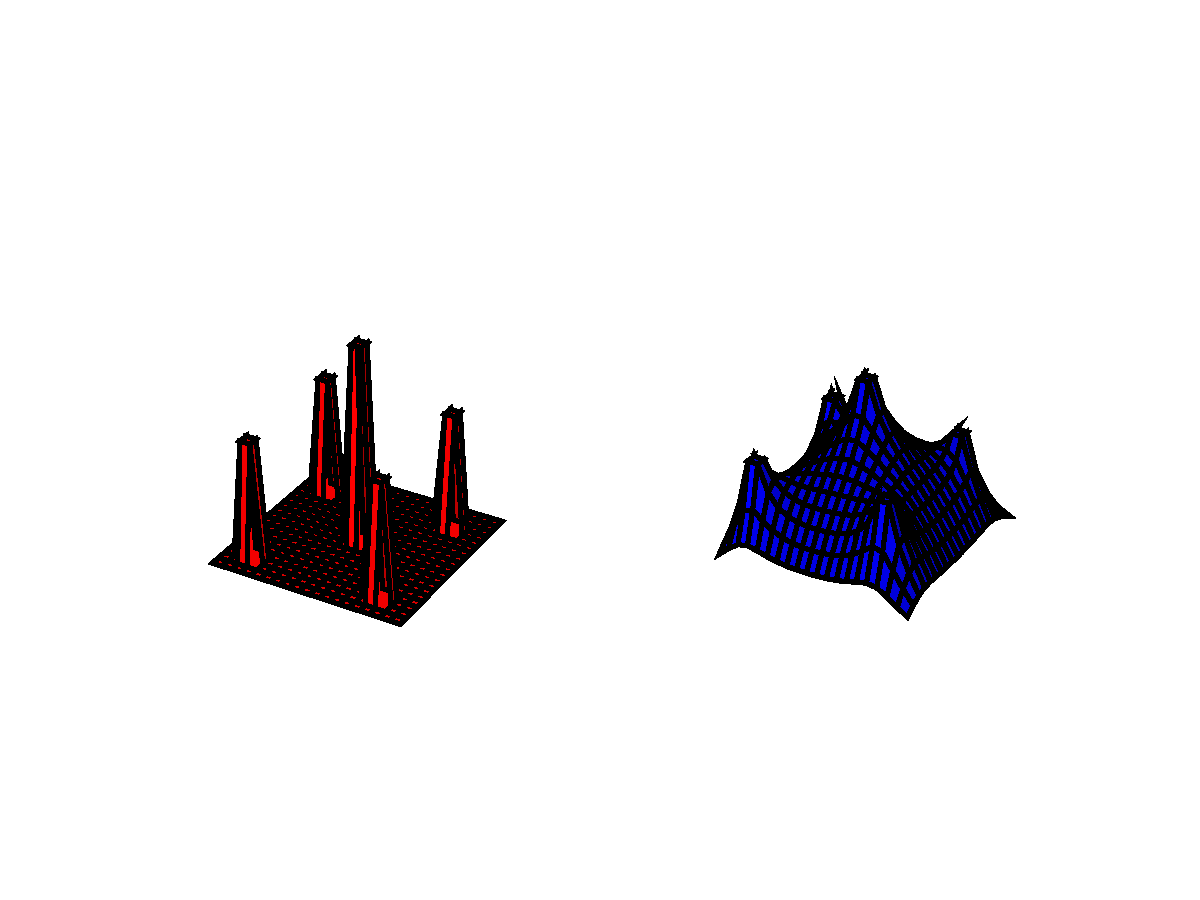
\includegraphics[width=\textwidth]{tent.pdf}
\caption{Tent pole configuration (left) and optimal elastic tent (right).}
\label{fig:tent}
\end{figure}

The following code is helpful in solving this problem. We first provide a method that calculates the matrix $H$.
\begin{lstlisting}
def laplacian(n):
    """
    Construct the discrete Dirichlet energy matrix H for an n x n grid.
    Inputs:
        n -- side length of grid
    Returns:
        dense array of shape n^2 x n^2
    """
    n = n+2
    data = -1*np.ones((5, (n-2)**2))
    data[2,:] = 4
    data[1, n-3::n-2] = 0
    data[3, ::n-2] = 0
    diags = np.array([-n+2, -1, 0, 1, n-2])
    return spar.spdiags(data, diags, (n-2)**2, (n-2)**2).todense()
\end{lstlisting}
Next, we initialize the tent pole configuration for a grid of side length $n$.
\begin{lstlisting}
>>> #create the tent pole configuration
>>> L = np.zeros((n,n))
>>> L[n/2-1:n/2+1,n/2-1:n/2+1] = .5
>>> m = [n/6-1, n/6, int(5*(n/6.))-1, int(5*(n/6.))]
>>> mask1, mask2 = np.meshgrid(m, m)
>>> L[mask1, mask2] = .3
>>> L = L.ravel()
\end{lstlisting}
An appropriate initial guess for $x, y$ and $\lambda$ is
\begin{lstlisting}
>>> #initial guess
>>> x = np.ones((n,n))
>>> x = x.ravel()
>>> y = np.ones(n**2)
>>> l = np.ones(n**2)
\end{lstlisting}
We leave it to you to initialize the vector $c$, the constraint matrix $A$ (it's just the identity matrix of
appropriate size), and to call the function \li{laplacian} to initialize the matrix $H$.
We can solve and plot the tent with the following code:
\begin{lstlisting}
>>> from matplotlib import pyplot as plt
>>> from mpl_toolkits.mplot3d import axes3d
>>> z = qInteriorPoint(H, c, A, L, (x,y,l), niter=10, verbose=False).reshape((n,n))
>>> #plot the solution
>>> dom = np.arange(n)
>>> X, Y = np.meshgrid(dom, dom)
>>> fig = plt.figure()
>>> ax1 = fig.add_subplot(111, projection='3d')
>>> ax1.plot_surface(X, Y, z,  rstride=1, cstride=1, color='r')
>>> plt.show()
\end{lstlisting}

\begin{problem}
Solve the circus tent problem with the tent pole configuration given above, for grid side length $n = 15$.
Plot your solution.
\end{problem}

\section*{Application: Markowitz Portfolio Optimization}
Suppose you have a certain amount of money saved up, with no intention of consuming it any time soon.
What will you do with this money? If you hide it somewhere in your living quarters or on your person,
it will lose value over time due to inflation, not to mention you run the risk of burglary or accidental
loss. A safer choice might be to put the money in a bank account. Here, there is less risk of losing the
money, plus you may even add to your savings through interest payments from the bank. You could also
consider purchasing bonds from the government or stocks from various companies, which come with their own
sets of risks and returns. Given all of these possibilities, how can you invest your money in such a way
that maximizes the return (i.e. the wealth that you gain over the course of the investment) while still
exercising caution and avoiding excessive risk? Economist and Nobel laureate Harry Markowitz developed
the mathematical underpinnings of and answer to this question in his work on modern portfolio theory.

A \emph{portfolio} is a set of investments over a period of time. Each
investment is characterized by a financial asset (such as a stock or bond) together with the proportion of
wealth allocated to the asset. An asset is a random variable, and can be described as a sequence of values over time.
The variance or spread of these values is associated with the risk of the asset, and the percent change of the values
over each time period is related to the return of the asset.
In the present treatment, we will assume that each asset has a positive risk, i.e.
there are no \emph{riskless} assets available.

Stated more precisely, our portfolio consists of $n$ risky assets together with an allocation vector
$x := (x_1,\ldots,x_n)^T$, where $x_i$ indicates the proportion of wealth we invest in
asset $i$. By definition, the vector $x$ must satisfy
\[
\sum_{i=1}^n x_i = 1.
\]
The $i$-th asset has an expected rate of return $\mu_i$ and a standard deviation $\sigma_i$.
The total return on our portfolio, i.e. the expected percent change in our invested wealth over the investment period,
is given by
\[
\sum_{i=1}^n \mu_ix_i.
\]
We define the risk of this portfolio in terms of the covariance matrix $Q$ of the $n$ assets:
\[
\sqrt{x^T Q x}.
\]
The covariance matrix $Q$ is always positive semidefinite, and captures the variance and correlations of the assets.

Given that we want our portfolio to have a prescribed return $\mu$, there are in general many possible allocation vectors $x$
that make this possible. It would be wise to choose the vector minimizing the risk. We can state this as a quadratic program:
\begin{align*}
\text{minimize }\qquad \frac{1}{2}&x^TQx\\
\text{subject to }\qquad &\sum_{i=1}^n x_i = 1,\\
&\sum_{i=1}^n \mu_ix_i = \mu.\\
\end{align*}
Note that we have slightly altered our objective function for convenience. Minimizing $\frac{1}{2}x^TQx$ is equivalent
to minimizing $\sqrt{x^T Q x}$.
The solution to this problem will give the portfolio with least risk having a return $\mu$. Because the components of $x$
are not constrained to be nonnegative, the solution may have some negative entries. This indicates short selling those
particular assets. If we want to disallow short selling, we simply include nonnegativity constraints, resulting in the
following problem:
\begin{align*}
\text{minimize }\qquad \frac{1}{2}&x^TQx\\
\text{subject to }\qquad &\sum_{i=1}^n x_i = 1,\\
&\sum_{i=1}^n \mu_ix_i = \mu,\\
&x \geq 0.
\end{align*}

Each return value $\mu$ can be paired with its corresponding minimal risk $\sigma$. If we plot these risk-return pairs on the
risk-return plane, we obtain a hyperbola. In general, the risk-return pair of any portfolio, optimal or not, will be found
in the region bounded on the left by the hyperbola. The positively-sloped portion of the hyperbola is known as the
\emph{efficient frontier}, since the points there correspond to optimal portfolios. Portfolios with risk-return
pairs that lie to the right of the efficient frontier are inefficient portfolios, since we could either
increase the return while keeping the risk constant, or we could decrease the risk while keeping the return
constant. See Figure \ref{fig:frontier}.

\begin{figure}
\centering
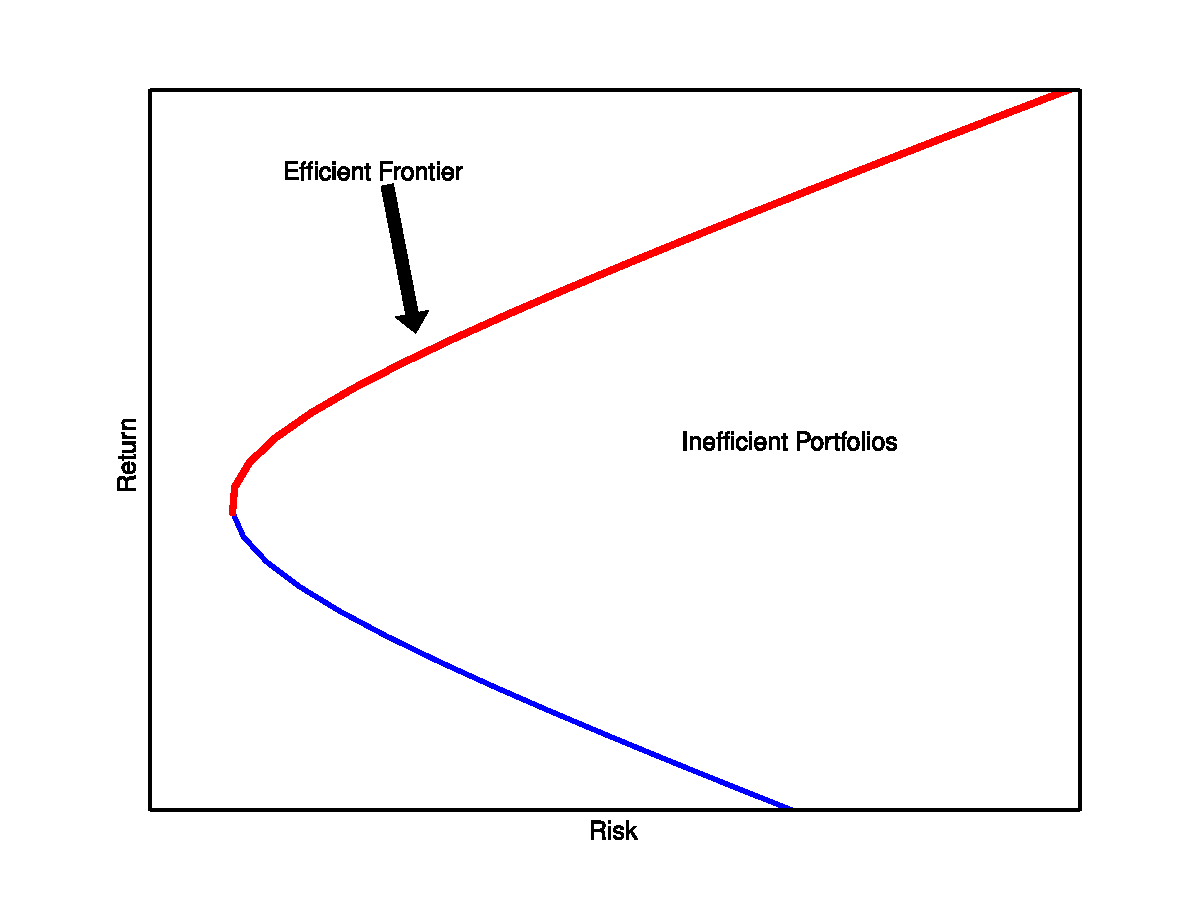
\includegraphics[width=\textwidth]{frontier.pdf}
\caption{Efficient frontier on the risk-return plane.}
\label{fig:frontier}
\end{figure}

One difficulty of this model is that the risk and return of each asset is in general unknown. After all, no one can predict the stock
market with complete certainty. There are various ways of estimating these values given past stock prices, and we take a very straightforward
approach. Suppose for each asset we have $k$ previous return values of the asset. That is, for asset $i$, we have the data vector
\[
y^i = [y^i_1,\,\, \ldots, \,\,y^i_k]^T.
\]
We estimate the expected rate of return for asset $i$ by simply taking the average of $y_1,\ldots,y_k$, and we estimate the variance
of asset $i$ by taking the variance of the data. We can estimate the covariance matrix for all assets by taking the covariance matrix of the
vectors $y^1,\ldots,y^n$. In this way, we obtain estimated values for $Q$ and $\mu_i$.

\begin{problem}
The text file \li{portfolio.txt} contains historical stock data for several assets (U.S. bonds, gold, S\&P 500, etc).
In particular, the first column gives the years corresponding to the data, and the remaining eight columns give the historical returns
of eight assets over the course of these years. Use this data to estimate the covariance matrix $Q$ as well as the expected rates
of return $\mu_i$ for each asset. Assuming that we want to guarantee an expected return of $\mu = 1.13$ for our portfolio,
find the optimal portfolio both with and without short selling.

Since the problem contains both equality and inequality constraints, use the QP solver in CVXOPT rather than your Interior Point method.

\end{problem} 